An example comment is taken from the standard library is seen in Figure~\ref{fig:odd}

\begin{figure}
    \begin{minted}{sml}
(*
==odd?==
***odd?***
** odd? :: Number -> Boolean **
odd? checks if a number is odd, 
 returning a __boolean__ value.
\#Example:\#
    > odd? 5
    > true : Boolean
    > odd? 4
    > false : Boolean
*)
    \end{minted}
    \caption{Markdown comment for the standard library function odd?}
\label{fig:odd}
\end{figure}

\begin{figure}
    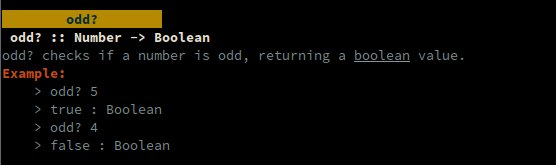
\includegraphics[width=\textwidth]{images/odd.jpg}
    \caption{odd? as seen in the terminal}
\label{fig:oddterm}
\end{figure}

\begin{itemize}
    \item a \textbf{comment} begins with `(*' and ends with `*)'
    \item the \textbf{comment name} is surrounded with `=='. This is the lookup string for the repl
        search.
    \item the \textbf{repl title} is surrounded with `***'. This text will be highlighted by a yellow
        bar in the repl.
    \item text to be rendered \textbf{bold} is surrounded with `**'
    \item text to be \underline{underlined} is surrounded with `__'
    \item headers are surrounded with `\#' 
    \item plain text is left without markup.
\end{itemize}

While not enforced by the syntax itself, underlined words are those which can be found in the
glossary. The glossary is a list of words, written with this markup, which might be unfamiliar to
students.
